\chapter{Supplementary Materials for Chapter III}
\author{Mohammad Y Karim, Eric I. Corwin}


\section{Forces on Grain Pile}
The lift force $F_{L}$ can be described by a simple model consisting of three parts: the horizontal component of the static load $F_{S}$, the horizontal component of the impact forces $F_{C}$, and the horizontal forces due to momentum transfer of outflowing particles $F_{flow}$.  

The static pile above the intruder has a mass proportional to the volume enclosed by the shock front and the intruder profile, shown by the grey region in Figure \ref{diagram}. For a given exponent $n$, the shape of the intruder profile is given by $g(x)=(1-x^n)^{1/n}$ and the shock front $f(x)$ given by Equation 5 in the main article. For a small segment of of the trapped area of width $dx$ and thickness $w_{cell}$ the volume $dV=w_{cell}[f(x)-g(x)]dx$. The net horizontal component of this weight is given by
\begin{equation} 
F_{S} = \int_0^1  w_{cell}  [f(x)-g(x)] \phi\rho_{g}g\cos(\alpha(x)) \sin(\alpha(x))dx
\label{fstatic}
\end{equation}
where the density of glass is $\rho_{g}=2500kg/m^3$, $g$ is gravitational acceleration and $\alpha(x)$ the angle between the horizontal and tangent to $g(x)$. This contribution is shown on Figure \ref{forcePlotSupplement} as the downward pointing triangles. We approximate the volume fraction $\phi=0.6$, slightly lower than random close packing because of the presence of confining walls in our system which is about 8 bead diameters thick. The cosine term gives the normal component to the tangent and the sine resolves the horizontal component. The horizontal component of the force is integrated over the length of the intruder to calculate the lift force due to the static pack. The integration limits are $x\in[0,1]$ where $x=0$ and $x=1$ are the left and right edges of the intruder respectively. 

The collisional force $F_{C}$ (upward pointing triangles on Figure \ref{forcePlotSupplement}) due to beads impacting the shock boundary and is given by 
\begin{equation} 
F_{C} = \int_0^1 \phi_{d}\rho_{g}w_{cell} [\vec{v}(x)\cdot \hat{n}(x)]^{2} \sin{\theta(x)}dx
\label{fcollision}
\end{equation}
where $\phi_{d}\rho_{g}w_{cell} \vec{v}(x)\cdot \hat{n}(x)dx$ is the incident mass per unit time at $x$ on a small segment $dx$ of the shock front. $\theta(x)$ is the angle between the horizontal and tangent to $f(x)$.  The normal component of the incident velocity of particles colliding with the shock front is given by $\vec{v}(x)\cdot \hat{n}(x)$. The velocities are obtained from PIV measurements of the flow field, as shown by a representative image of the field overlaid on the intruder in Figure \ref{flowField}. The fraction of space occupied by freely falling particles is $\phi_{d}\approx0.03$ as measured directly from the images. Assuming that collisions are inelastic, the rate of momentum transfer normal to $f(x)$ is $\phi_{d}\rho_{g}w_{cell} \left(\vec{v}(x)\cdot \hat{n}(x)dx \right) \left(\vec{v}(x)\cdot \hat{n}(x)\right)\sin\theta(x)$. The sine term comes from the horizontal component of this force at $g(x)$.

The horizontal reaction force $F_{flow}$ (represented by diamonds on Figure \ref{forcePlotSupplement}) on the intruder due to mass ejection from the granular pile  is 
\begin{equation} 
F_{flow} =  \phi \rho w_{cell} \left( \left[ f(1)-g(1) \right] v_{x,1}^{2} - \left[ f(0)-g(0) \right] v_{x,0}^{2} \right)
\label{fflow}
\end{equation}
where $\phi \rho w_{cell}([f(x_0)-g(x_0)] v^{2}$ is the horizontal momentum transferred due to particles being ejected from the area between $f(x_0)$ and $g(x_0))$. The velocities $v_{x,0}$ and $v_{x,1}$ are the mean horizontal bead velocities exiting the cross-section $w_{cell}[f(x)-g(x)]$ at $x=0$ and $x=1$ respectively. The volume fraction is $\phi=0.6$. 


\begin{figure*}
	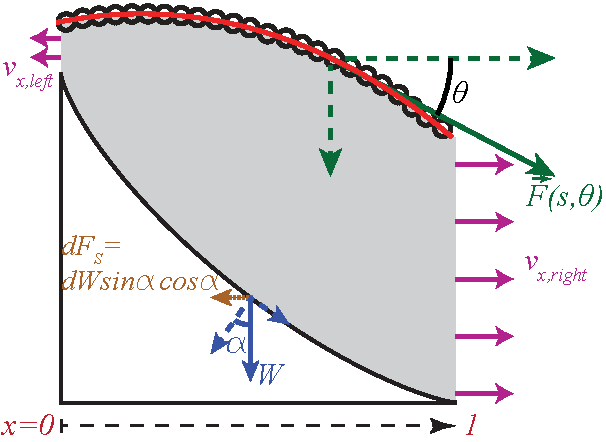
\includegraphics[width=\textwidth]{Figures/chapter3sup/diagramSupplement}
	\caption{Diagram of force vectors and velocites used to calculated $F_{L}$.}
	\label{diagram}
\end{figure*}

\begin{figure*}
	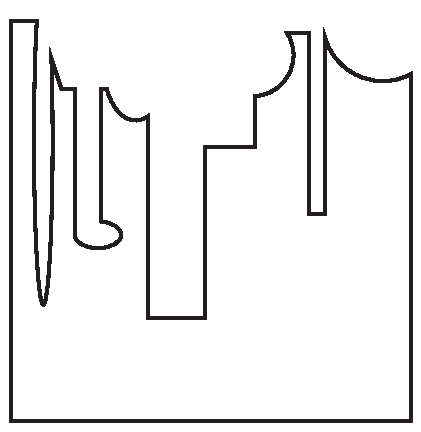
\includegraphics[width=\textwidth]{Figures/chapter3sup/randomShape}
	\caption{Illustration of the intruder with random features on the leading edge. The shock front from this shape still maintains the catenary shape.}
	\label{randomShape}
\end{figure*}

\begin{figure*}[h]
	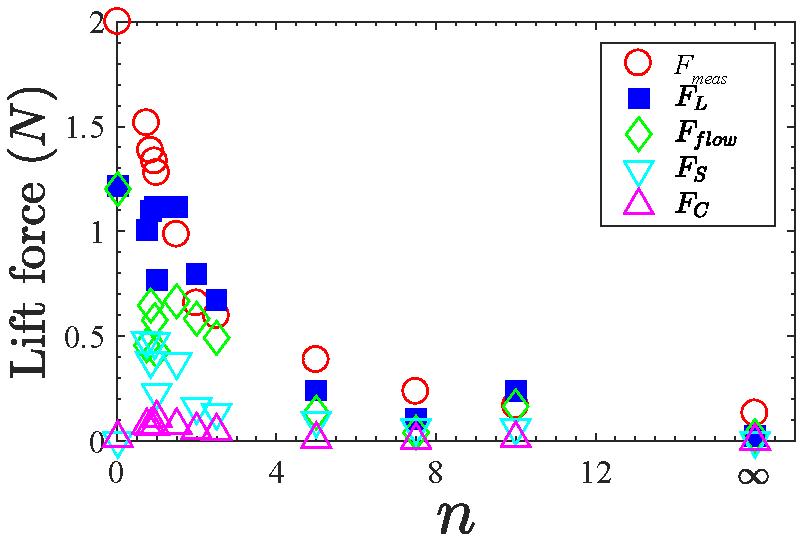
\includegraphics[width=\textwidth]{Figures/chapter3sup/forcePlotSupplement}
	\caption{Plots of total measured lift force $F_{meas}$, calculated lift force $F_L$ (blue squares), force due to mass ejection from trapped pile $F_{flow}$ (green diamond), quasi-static load contribution $F_S$ (downward pointing arrow), and force due to impacts $F_C$ (upward pointing arrow) as a function of $n$.}
	\label{forcePlotSupplement}
\end{figure*}

\begin{figure*}
	\includegraphics[width=\textwidth]{Figures/chapter3sup/supplementQuiver}
	\caption{Representative mean flow field around an intruder with super-disk exponent $n=0.75$. The white masked out region is the intruder and the arrows are velocity vectors.}
	\label{flowField}
\end{figure*}